\label{method_altitude}

\subsection{Ước tính độ cao bằng khí áp kế kết hợp với bộ đếm bước và HAR}

\begin{figure}[b!]
    \centering
    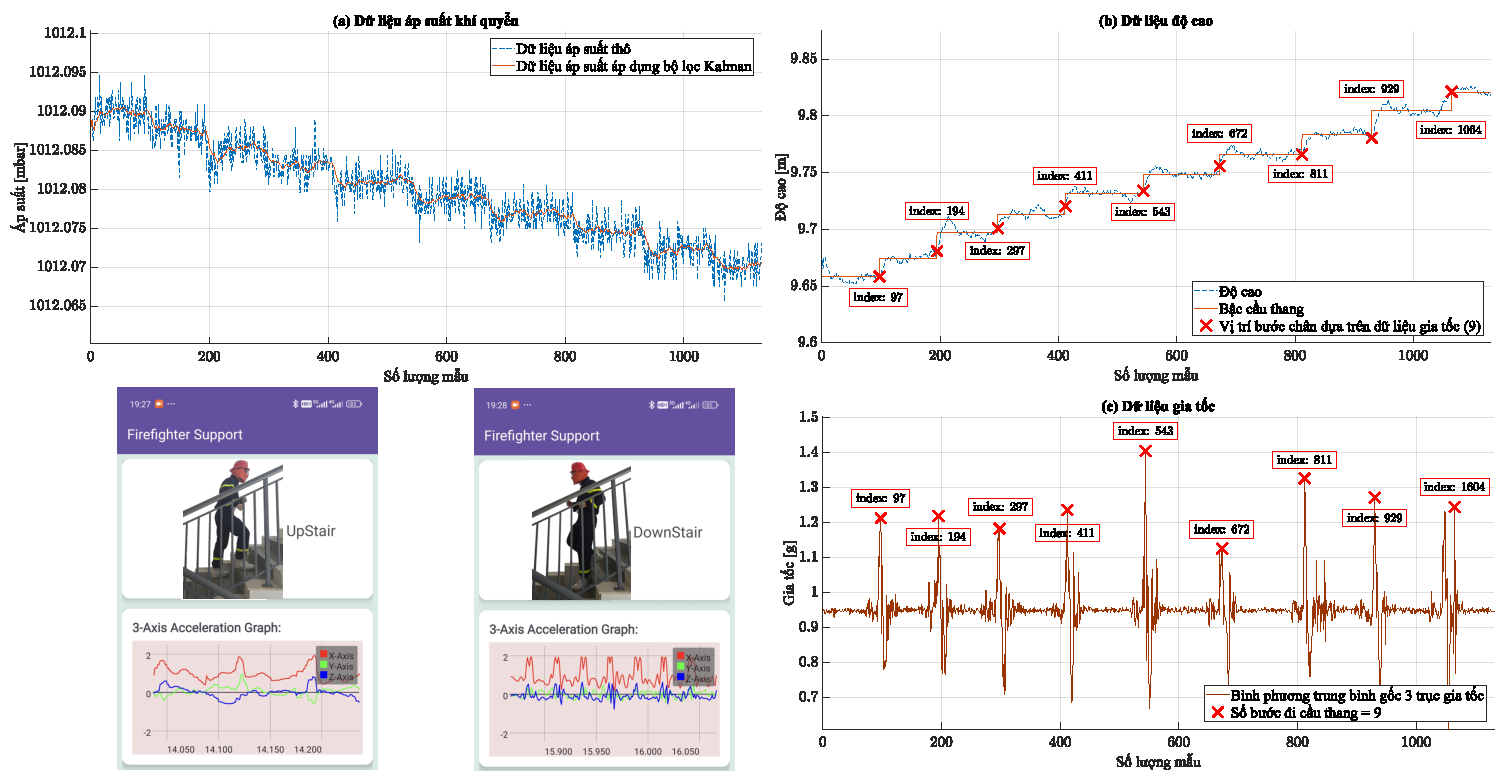
\includegraphics[width=1\linewidth]{Figure/pressure_altitude.pdf}
    \caption{Hình ảnh hóa dữ liệu (a) Áp suất khí quyển, (b) Độ cao và (c) Gia tốc kết hợp với bộ đếm bước và (d) nhận dạng hoạt động con người}
    \label{pressure_altitude}
\end{figure}

Trong các hệ thống định vị trong nhà dựa trên IMU, cảm biến áp suất khí quyển thường được sử dụng để ước lượng độ cao, nhằm cung cấp góc nhìn không gian 3D cho vị trí của người cứu hộ. Trong hệ thống này, khí áp kế GY-37 tích hợp trên mô-đun gắn tại thắt lưng đo sự thay đổi áp suất khí quyển để suy ra thay đổi về độ cao. Tuy nhiên, việc sử dụng cảm biến áp suất trong môi trường cứu hộ trong nhà phức tạp đặt ra nhiều thách thức. Ví dụ, các hệ thống tăng áp thường được lắp trong buồng thang bộ, hoặc nhiệt độ khắc nghiệt trong các tình huống cháy có thể gây ra sự dao động áp suất đáng kể~\cite{yuan2016research}. Những yếu tố này dẫn đến nhiễu lớn trong phép đo, làm sai lệch đáng kể kết quả ước lượng độ cao.

Để khắc phục những hạn chế này, hệ thống được đề xuất tích hợp bộ lọc Kalman vào đường ống xử lý tín hiệu (Hình~\ref{pressure_altitude}a) để loại bỏ nhiễu và ổn định các chỉ số áp suất trước khi tính toán độ cao. Điều quan trọng là hệ thống không chỉ dựa vào dữ liệu khí quyển. Bằng cách tận dụng HAR, đặc biệt là các thuật toán đếm bước chân và phát hiện đỉnh được áp dụng cho tín hiệu gia tốc (Hình~\ref{pressure_altitude}c), hệ thống xác định chính xác thời điểm người ứng cứu đang lên hoặc xuống cầu thang. Việc nhận biết các hoạt động liên quan đến cầu thang là rất quan trọng, vì nó cho phép hệ thống phân biệt giữa chuyển động thẳng đứng thực tế và các hiện tượng nhiễu do biến đổi áp suất.

Dựa trên các sự kiện leo cầu thang và vị trí bước chân được phát hiện (Hình~\ref{pressure_altitude}b), số bước chân được thực hiện sẽ được suy ra. Số bước chân này, kết hợp với các thay đổi độ cao được tính toán dựa trên áp suất, cho phép hệ thống ước tính khoảng cách thẳng đứng đã đi qua và xác định độ cao cụ thể của tầng nơi người phản hồi đang ở. Giao diện ứng dụng hiển thị trạng thái lên và xuống cầu thang cùng với biểu đồ gia tốc theo thời gian thực, hỗ trợ nhận thức tình huống. Sự kết hợp giữa dữ liệu khí áp và HAR này giúp tăng cường độ chính xác của ước tính độ cao, đảm bảo định vị chính xác ở tầng ngay cả trong điều kiện vận hành khó khăn.